\section{Workload Details}
\label{app:workload-detail}

\autoref{tab:workload-detail} lists the shape, dtype and reference for the five expert kernels
and five transfer targets on each platform. Expert kernels are the sources from which
\sys{} induces skills; transfer targets contribute no lineage.

\begin{table*}[h]
  \centering
  \small
  \setlength{\tabcolsep}{5pt}
  \begin{tabular}{@{}llp{0.40\textwidth}l@{}}
    \toprule
    \textbf{Role} & \textbf{Kernel} & \textbf{Shape (dtype)} & \textbf{Reference} \\
    \midrule
    \multicolumn{4}{@{}l}{\textit{NVIDIA --- expert kernels}} \\
    source & GEMM   & $M{=}N{=}K{=}4096$ (BF16) & cuBLAS \\
    source & Conv2d & $N{=}8$, $C{=}64$, $H{=}W{=}56$, $F{=}128$, $K{=}3$, s${=}1$, p${=}1$ (FP16) & cuDNN \\
    source & FMHA   & batch $8$, heads $64$, seq $2048$, dim $128$ (FP16) & FlashInfer \\
    source & GDN    & $h_{qk}{=}16$, $h_v{=}48$, dim $128$, chunk $64$, seq $4096$ (BF16) & FlashInfer / FLA \\
    source & Top-K  & batch $64$, seq $4096$, top-$k{=}512$ (FP32) & FlashInfer \\
    \multicolumn{4}{@{}l}{\textit{NVIDIA --- transfer targets}} \\
    target & KDA               & batch $1$, tokens $4096$, heads $96$, dim $128$ (BF16) & FLA \\
    target & Sparse Attention  & queries $8192$, heads $128$, $2048$ sparse indices & FlashInfer \\
    target & Top-P             & batch size $32$, vocabulary $128256$ & FlashInfer \\
    target & Fused Add-RMSNorm & batch size $8192$, hidden $7168$ & Torch \\
    target & GQA               & tokens $16384$, $32$ query / $8$ KV heads & FlashInfer \\
    \midrule
    \multicolumn{4}{@{}l}{\textit{Ascend --- expert kernels}} \\
    source & GEMM   & $M{=}N{=}K{=}4096$ (BF16) & Torch-NPU  \\
    source & Conv2d & $N{=}8$, $C{=}64$, $H{=}W{=}56$, $F{=}128$, $K{=}3$, s${=}1$, p${=}1$ (FP16) & AscendC custom op \\
    source & FMHA   & batch $8$, heads $64$, seq $2048$, dim $128$ (FP16) & Torch-NPU  \\
    source & GDN    & $h_{qk}{=}16$, $h_v{=}48$, dim $128$, chunk $64$, seq $4096$ (BF16) & vLLM-Ascend \\
    source & Top-K  & batch $64$, seq $4096$, top-$k{=}512$ (FP32) & Torch-NPU  \\
    \multicolumn{4}{@{}l}{\textit{Ascend --- transfer targets}} \\
    target & KDA               & batch $1$, tokens $4096$, heads $96$, dim $128$ (BF16) & Torch-NPU \\
    target & Sparse Attention  & queries $8192$, heads $128$, $2048$ sparse indices & AscendC custom op \\
    target & Top-P             & batch size $32$, vocabulary $128256$ & Torch-NPU \\
    target & Fused Add-RMSNorm & batch size $8192$, hidden $7168$ & Torch-NPU \\
    target & GQA               & tokens $16384$, $32$ query / $8$ KV heads & AscendC custom op \\
    \bottomrule
  \end{tabular}
  \caption{The workload suite separates five expert kernels used for induction from five targets used for transfer on each platform.}
  \label{tab:workload-detail}
\end{table*}

\section{Source-Tier Reconstruction and Memory-Based Kernel Agents}
\label{sec:exp-cuda}

This appendix backs \autoref{fig:cuda-bars} with absolute latencies, cost trajectories and the
per-step record of one baseline run. AdaExplore~\citep{adaexplore} builds failure-rule memory with
MCTS-style exploration; AccelOpt~\citep{accelopt} maintains an LLM-summarized memory over generated
kernels. Both are re-run in our harness with their search policy and memory schema preserved
(\autoref{sec:appendix-baselines}). These numbers are a reconstruction check, not a transfer claim:
the operators here are the ones whose lineages the library was built from.


\section{Main-Tier Per-Instance Latencies}
\label{app:tables}

\autoref{tab:appendix-cuda-latencies} gives the absolute per-kernel latencies behind
\autoref{fig:cuda-bars}. ``FAIL'' indicates that the method did not produce a correct
kernel within the budget; $\dagger$ marks a post-hoc adapter audit rather than an
as-submitted valid kernel.

\begin{table*}[h]
  \centering
  \small
  \setlength{\tabcolsep}{6pt}
  \begin{tabular}{@{}llrrrr@{}}
    \toprule
    \textbf{Platform} & \textbf{Kernel} & \textbf{\sys{} (ms)} & \textbf{AdaExplore (ms)} & \textbf{AccelOpt (ms)} & \textbf{Reference (ms)} \\
    \midrule
    SM90  & GEMM   & 0.3130  & 0.3198   & 0.3190  & 0.3086 \\
    SM90  & Conv2d & 0.0157  & 0.0684   & 0.0658  & 0.0272 \\
    SM90  & FMHA   & 3.5183  & FAIL     & 5.1499  & 3.3121 \\
    SM90  & GDN    & 0.2439  & 17.7673  & FAIL    & 0.2816 \\
    SM90  & Top-K  & 0.0143  & 0.1338   & 0.1276  & 0.0160 \\
    \midrule
    SM120 & GEMM   & 0.3681  & 0.3896   & 0.3933  & 0.3688 \\
    SM120 & Conv2d & 0.0235  & 0.0760$^\dagger$ & 0.0822  & 0.0253 \\
    SM120 & FMHA   & 3.2151  & FAIL     & 3.6366  & 3.1932 \\
    SM120 & GDN    & 0.6348  & FAIL     & FAIL    & 0.6867 \\
    SM120 & Top-K  & 0.0131  & FAIL     & 0.0288  & 0.0169 \\
    \bottomrule
  \end{tabular}
  \caption{\sys{} produces correct kernels on all ten CUDA workloads, while AdaExplore and AccelOpt fail on four and two, respectively.}
  \label{tab:appendix-cuda-latencies}
\end{table*}

\paragraph{Expert-source comparison.}
\autoref{tab:expert-source-ablation} gives the per-workload reconstruction latencies for the comparison in \autoref{sec:exp-source-ablation}. The Gen. column denotes expert-source prompting, and slowdown is its latency divided by the corresponding \sys{} latency.

\begin{table}[t]
  \centering
  \small
  \setlength{\tabcolsep}{6pt}
  \begin{tabular}{@{}llrrr@{}}
    \toprule
    \textbf{Platform} & \textbf{Kernel} & \textbf{Gen. (ms)} & \textbf{\sys{} (ms)} & \textbf{Slowdown} \\
    \midrule
    SM90  & GEMM   & 0.4070  & 0.3130 & $1.30\times$ \\
    SM90  & Conv2d & 0.2273  & 0.0157 & $14.48\times$ \\
    SM90  & FMHA   & 27.7556 & 3.5183 & $7.89\times$ \\
    SM90  & GDN    & 25.6522 & 0.2439 & $105.18\times$ \\
    SM90  & Top-K  & 0.0211  & 0.0143 & $1.48\times$ \\
    \midrule
    SM120 & GEMM   & 0.4781  & 0.3681 & $1.30\times$ \\
    SM120 & Conv2d & 0.1369  & 0.0235 & $5.83\times$ \\
    SM120 & FMHA   & 11.8063 & 3.2151 & $3.67\times$ \\
    SM120 & GDN    & 23.7612 & 0.6348 & $37.43\times$ \\
    SM120 & Top-K  & 0.0147  & 0.0131 & $1.12\times$ \\
    \bottomrule
  \end{tabular}
  \caption{Conditioned skills outperform direct expert-source prompting on all ten CUDA workloads under the same \$10 budget.}
  \label{tab:expert-source-ablation}
\end{table}

% \section{Baseline Re-implementation Notes}
% \label{sec:appendix-baselines}

\paragraph{Cost over the budget.}
\autoref{fig:budget-curves} reads the same comparison as a function of cumulative LLM-API cost on
SM120. Loading the induced library costs around $\$0.7$ in retrieval and load --- the flat plateau
at the start of each \sys{} curve --- and is paid once per workload, since lineages and SkillCards
stay in a single prefix-cached chat session. After the load, \sys{} reaches its eventual best
between $\$4$ and $\$7$, well under the cap, and each step lines up with one named, verified skill
rather than a black-box submission.

\begin{figure*}[t]
\centering
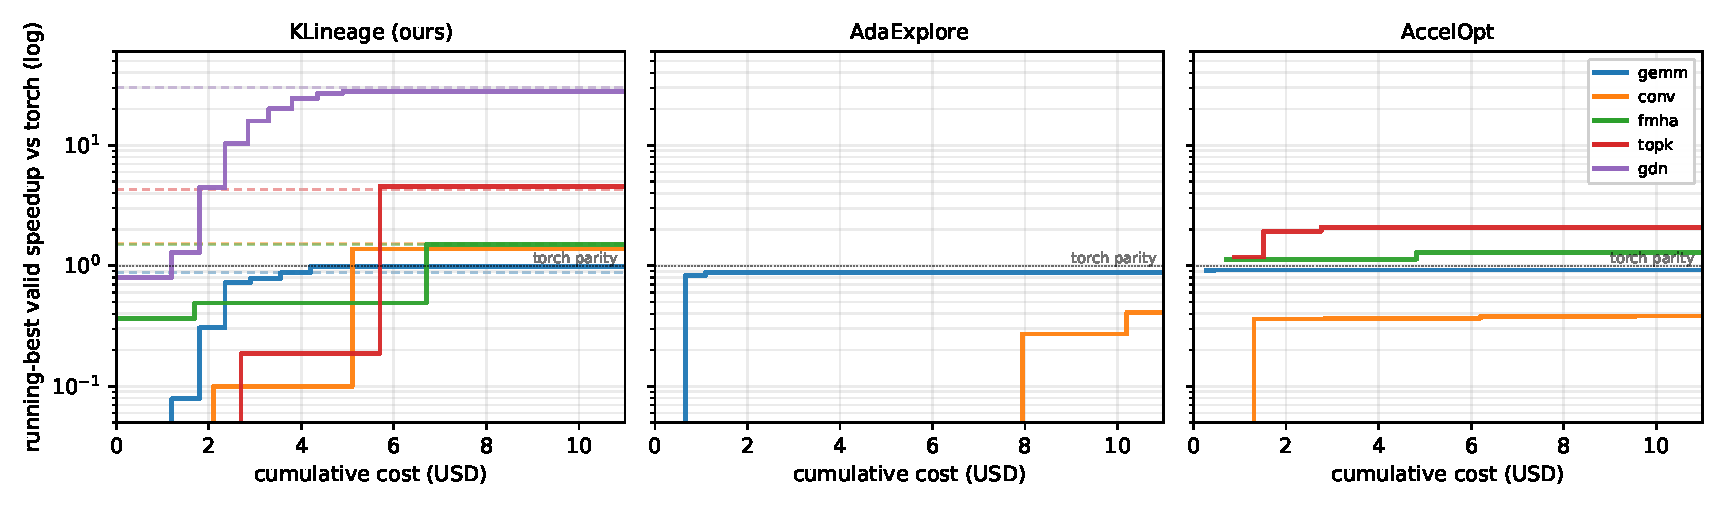
\includegraphics[width=\textwidth]{budget_curves.pdf}
\caption{\sys{} reaches its best SM120 kernels within \$4--\$7 of online optimization cost.}
\label{fig:budget-curves}
\end{figure*}

% We re-run AdaExplore~\citep{adaexplore} and AccelOpt~\citep{accelopt} under the same evaluation harness, the same Claude Opus 4.6 backbone, and the same per-workload \$$10$ optimization-cost budget used by \sys (\autoref{sec:exp-setup}). Both baselines submit through the same compile/correctness/profile gate and are scored against the same vendor reference (\autoref{tab:workloads}). This appendix records what is preserved from each published system and what was necessarily adapted, so that the head-to-head comparison can be reproduced.

% \paragraph{AdaExplore (failure-rule MCTS memory).}
% We reuse the public AdaExplore configuration: failure-rule memory keyed by an extracted failure tag, MCTS-style exploration over an action vocabulary that matches our deoptimization categories, and per-step prompt templates supplied by the released code. The only adaptations are (i) routing all submissions through our harness so that compile/correctness/profile statuses are computed by the same evaluator used for \sys, and (ii) replacing the original budget (a fixed step count) with the cost budget so that all three methods are bounded by the same dollar amount on the same backbone. Failure-rule memory is reset at the start of every workload so that a previous workload's rules cannot leak into the next; this matches the published per-task semantics. We do not modify the search policy, the rule-extraction prompt, or the action vocabulary.

% \paragraph{Filtering out non-kernel wrappers.}
% Across the SM120 AdaExplore runs, several submissions reach the evaluator as wrapper programs: the agent emits a Triton kernel definition, but the surrounding \texttt{ModelNew} catches the kernel-call failure and returns the PyTorch reference. Such submissions can pass correctness and even report a nontrivial speedup, but the measured program is no longer the generated kernel. We confirmed this by rewriting the wrapper's reference-return path into a \texttt{raise}; under the same workload interface, these submissions no longer pass. As a post-hoc audit, we also wired a thin adapter that calls the underlying Conv2d kernels directly with the case-side $(x,w)$ tensors, bypassing the wrapper. This audit recovers two real kernels, but they are much slower than cuDNN (best about $0.41\times$ vs.\ torch and $0.33\times$ vs.\ cuDNN near the end of the run) and require an adapter not produced by AdaExplore's workflow. We therefore mark the SM120 Conv2d number with $\dagger$ in \autoref{tab:appendix-cuda-latencies}: it credits the real audited kernel, not the wrapper's near-parity score. We do not further edit AdaExplore submissions into new task-specific workflows, since such harness-level repair is not an operation organized by the published AdaExplore loop within the shared budget. AccelOpt and \sys do not produce this wrapper pattern in our runs.

% \paragraph{AccelOpt (LLM-summarized memory).}
% For AccelOpt we keep the per-step memory-summary prompt and the iterative refine-with-summary loop from the released system. Memory state is initialized empty per workload, identical to the published per-task semantics. As with AdaExplore, the only adaptations are routing submissions through our evaluator and using the cost budget. We do not introduce skill cards, lineage retrieval, or any \sys-specific memory schema into AccelOpt; its memory remains an LLM-summarized rolling state over the agent's own forward submissions.

% \paragraph{What is shared with \sys.}
% All three methods share the backbone (Claude Opus 4.6), the per-workload cost budget (\$$10$ USD), the evaluator (\texttt{triton.testing.do\_bench}, $100$ reps after $25$ warm-ups), the correctness check (three random seeds), the speedup definition ($T_{\mathrm{ref}}/T_{\mathrm{gen}}$), and the run count ($5$ runs per workload reported as the success-only geometric mean). The vendor reference is the same per platform: cuBLAS for GEMM, cuDNN for Conv2d, FlashInfer for FMHA / Top-K, and FlashInfer or FLA for GDN (\autoref{tab:workloads}). The only thing that varies across methods is the memory representation each one carries between submissions inside a single run.

% \paragraph{What is not preserved.}
% We do not run either baseline beyond \$$10$ in this submission, so we cannot rule out that further dollars would close the gap on individual workloads. We also do not introduce post-training: AdaExplore's failure-rule store and AccelOpt's summarized memory are both held in-context within a single workload's run and discarded between workloads, identical to the published per-task semantics. Per-workload absolute latencies for both baselines are listed alongside \sys in \autoref{tab:appendix-cuda-latencies}.

\section{Baseline Execution and Harness Notes}
\label{sec:appendix-baselines}

We evaluate AdaExplore~\citep{adaexplore} and AccelOpt~\citep{accelopt} in the same external harness used for \sys. This harness standardizes the parts that determine the reported score---input shapes, correctness tests, profiling, vendor references, and cost accounting---while preserving each baseline's own search policy and memory representation. In other words, we do not replace either baseline with a \sys-style memory or planner; each method still decides what to submit using its original in-context state.

All three methods use Claude Opus 4.6 as the online materialization backbone, the per-workload \$$10$ optimization-cost budget, the same compile/correctness/profile gate, and the same vendor reference per platform (\autoref{sec:exp-setup}, \autoref{tab:workload-detail}). We use a dollar budget rather than a fixed submission count because the methods differ in session structure and cache reuse: \sys keeps one prefix-cached chat session per workload, whereas the baselines either restart sessions per submission or use looser caching. The goal is therefore to compare optimization usefulness under the same online cost, not to measure each method's asymptotic ceiling under an unconstrained search horizon.

\paragraph{AdaExplore.}
For AdaExplore, we use the released failure-rule memory, failure-tag extraction, MCTS-style exploration, action vocabulary, and per-step prompt templates. The failure-rule memory is reset at the start of each workload, matching the published per-task setting and preventing rules from one workload from leaking into another. The only harness-level changes are that submissions are routed through our evaluator and budget meter, so that compile status, correctness, latency, and LLM cost are measured consistently with \sys and AccelOpt. We do not modify AdaExplore's search policy, rule-extraction prompt, or memory schema.

\paragraph{Non-kernel wrapper outputs.}
A practical issue arises in some AdaExplore runs: several submissions reach the evaluator as wrapper programs rather than executable generated kernels. The agent emits a Triton kernel definition, but the surrounding \texttt{ModelNew} catches the kernel-call failure and returns the PyTorch reference. Such submissions can pass correctness, and may even appear fast, but the measured program is then the fallback reference path rather than the generated kernel. We verified this by replacing the fallback return path with a \texttt{raise}; under the same workload interface, these submissions no longer pass.

We therefore exclude fallback-wrapper scores from the generated-kernel comparison. To avoid under-crediting AdaExplore, we additionally perform a post-hoc audit for SM120 Conv2d by wiring a thin adapter that directly calls the underlying generated Conv2d kernels with the case-side $(x,w)$ tensors. This audit recovers two real kernels, but they are much slower than cuDNN (best about $0.41\times$ vs.\ torch and $0.33\times$ vs.\ cuDNN near the end of the run), and the adapter itself is not produced by AdaExplore within its workflow. We mark this number with $\dagger$ in \autoref{tab:appendix-cuda-latencies}: it credits the real audited kernel rather than the wrapper's fallback score. We do not otherwise repair AdaExplore submissions or introduce task-specific adapters, since such harness-level repair is outside the published AdaExplore loop and the shared budget.

\paragraph{AccelOpt.}
For AccelOpt, we use the released iterative refine-with-summary loop and its per-step memory-summary prompt. The memory state is initialized empty for each workload, matching the published per-task setting. As with AdaExplore, submissions are routed through our evaluator and budget meter, but the baseline's memory remains an LLM-summarized rolling state over its own forward submissions. We do not introduce SkillCards, lineage retrieval, expert-derived transitions, or any \sys-specific memory schema into AccelOpt.

\paragraph{Shared scoring protocol.}
All three methods share the online backbone, the per-workload cost budget, the evaluator (\texttt{triton.testing.do\_bench} with \texttt{warmup=25} and \texttt{rep=100}, both in milliseconds), the correctness check (three random seeds), the speedup definition ($T_{\mathrm{ref}}/T_{\mathrm{gen}}$), and the run count ($5$ runs per workload, reported as success-only geometric mean). The vendor reference is fixed per platform and workload: cuBLAS for GEMM, cuDNN for Conv2d, FlashInfer for FMHA and Top-K, and FlashInfer or FLA for GDN (\autoref{tab:workload-detail}). Thus, the comparison keeps the model, evaluator, budget, and references fixed; what varies is the optimization memory each method carries between submissions.

\paragraph{Scope of the comparison.}
This comparison evaluates fixed-cost online optimization, not unlimited-horizon search. Search-heavy methods may improve with additional budget, and \sys could also use additional budget for repair and local exploration. Our goal in the main comparison is to ask how useful each memory representation is under the same online materialization cost and validation gate. Per-workload absolute latencies for both baselines are listed alongside \sys in \autoref{tab:appendix-cuda-latencies}.

\paragraph{What an AdaExplore trajectory looks like at the step level.}
\autoref{fig:ada-detail} shows the per-step trajectory for two of the AdaExplore SM120 cases. Panel (a) is GEMM, where $21$ valid kernels are produced over the $\$10$ budget at speedups ranging from $0.57\times$ to $0.88\times$, plus $8$ failed steps; the running-best reaches $0.88\times$ at $\$1.1$ and stays flat afterwards, and most subsequent valid kernels regress below the running-best rather than improve it. Panel (b) is Conv2d, where most steps fail outright ($16$ failed) or emit non-kernel wrappers that compute the right answer through PyTorch ($6$ flagged in the raw trajectory). A thin post-hoc adapter can benchmark two underlying kernels as real Conv2d kernels, reaching about $0.41\times$ near the end of the run, while the remaining wrappers are excluded. The two panels jointly motivate why we report running-best over a wrapper-filtered step set rather than picking the wrapper's reported speedup at face value: the latter would have credited the Conv2d wrappers with about $0.96\times$ on this case.

Green circles denote valid submissions, green diamonds denote adapter-audited kernels, red crosses denote excluded fallback wrappers, and grey triangles denote failed steps. The blue line tracks the best wrapper-filtered speedup, including the audited Conv2d kernels.

\begin{figure*}[h]
\centering
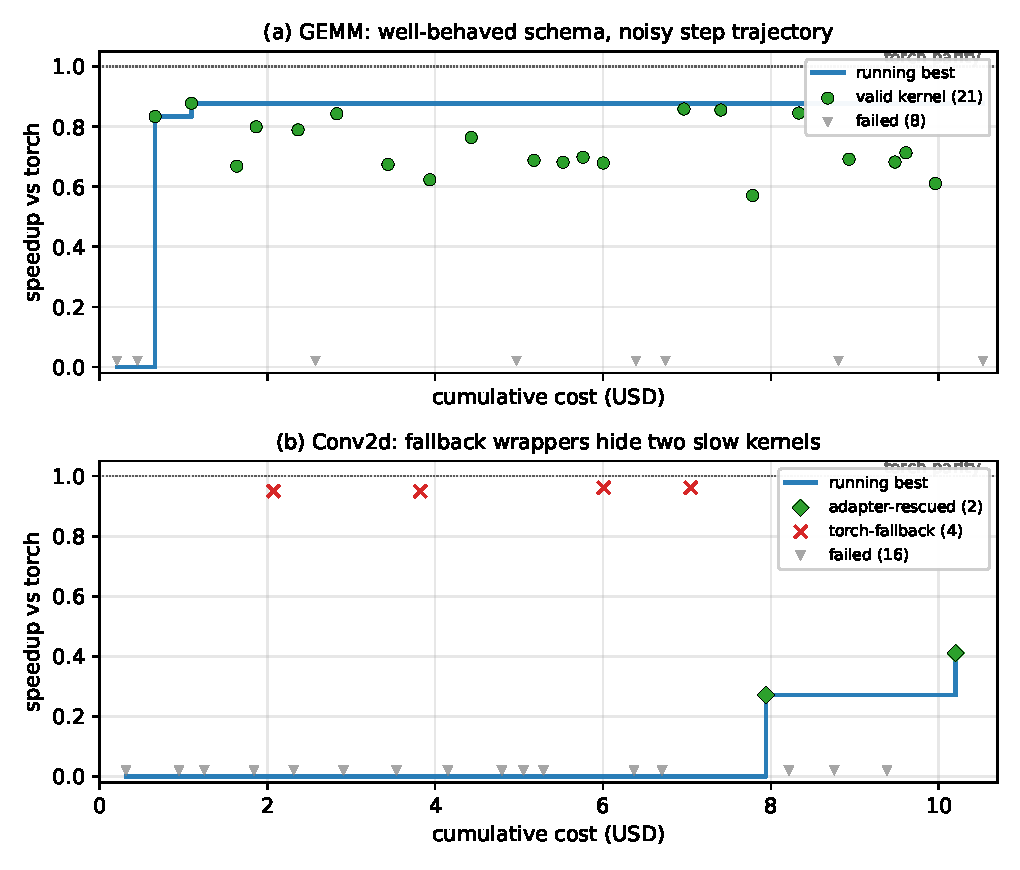
\includegraphics[width=0.78\textwidth]{budget_curve_ada_detail.pdf}
\caption{AdaExplore's SM120 trajectories show repeated regressions on GEMM and frequent failures or fallback wrappers on Conv2d.}
\label{fig:ada-detail}
\end{figure*}


\section{CUDA and Ascend Trajectories against Tokens and Cost}
\label{app:transfer-axes}

\autoref{fig:transfer-staircase} shows the CUDA and Ascend transfer trajectories against wall-clock time in the top and bottom panels, respectively. Each operator is normalized by the best kernel reached without \sys{}, except Ascend Sparse Attention, which uses the eager reference because the run without \sys{} produced no valid kernel.
To complement the time-based view, \autoref{fig:transfer-tokens} and \autoref{fig:transfer-cost} plot the same runs against cumulative API tokens and monetary cost, respectively, with CUDA above Ascend in each figure. Token counts include input and output tokens, including cache hits; normalization and shading follow the corresponding wall-clock plots.
These axes better capture agent-side optimization effort when a session is idle, interrupted, or resumed, where wall-clock time may not faithfully reflect the amount of model interaction.

For the cost analysis, we compute API cost using the DeepSeek V4.1-Flash peak rates: \$$0.30$ per million cache-miss input tokens, \$$0.006$ per million cache-hit input tokens, and \$$1.20$ per million output tokens, charged per API call.
This provides an upper bound on the actual cost of these runs, since only the Sparse Attention pair was executed during the peak-pricing window.

\begin{figure*}[h]
\centering

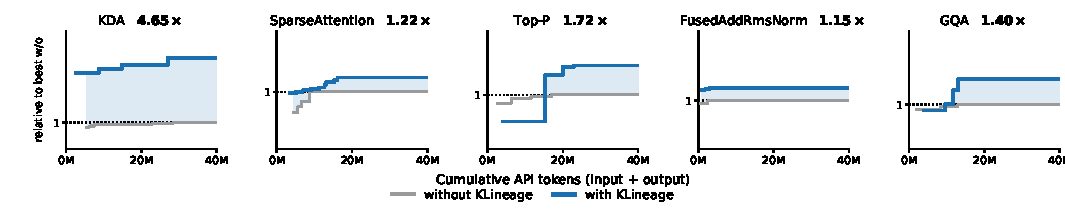
\includegraphics[width=\textwidth]{cuda_ab_tokens.pdf}

\vspace{4pt}

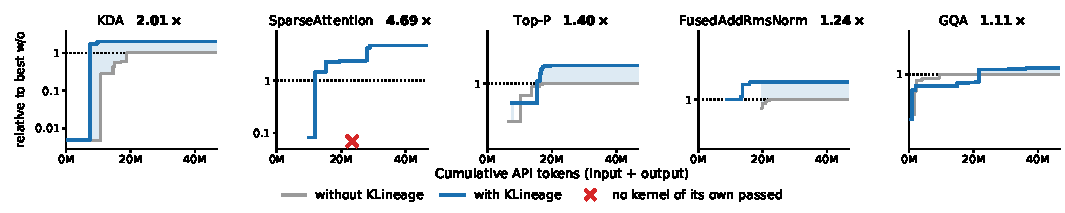
\includegraphics[width=\textwidth]{ascend_ab_tokens.pdf}

\caption{Token-based trajectories show the transfer gains from conditioned skills on both CUDA and Ascend.}
\label{fig:transfer-tokens}
\end{figure*}

\begin{figure*}[h]
\centering

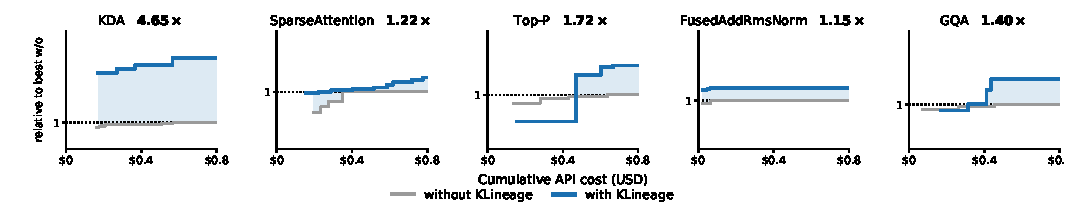
\includegraphics[width=\textwidth]{cuda_ab_cost.pdf}

\vspace{4pt}

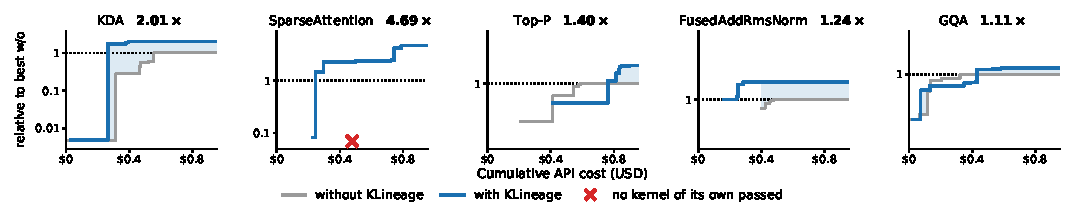
\includegraphics[width=\textwidth]{ascend_ab_cost.pdf}

\caption{Transfer trajectories against API cost show faster final kernels with conditioned skills on both platforms.}
\label{fig:transfer-cost}
\end{figure*}

\section{AscendC Technique Matrix}
\label{app:technique-matrix}

\autoref{tab:technique-matrix} audits the final submission of each setting on the five Ascend transfer
targets for the optimization mechanisms visible in its source. A mechanism is counted when its
implementation is present in the selected bundle; the audit describes code, not an isolated
performance effect, and it does not establish that any one mechanism caused a speedup. The setting with
\sys{} contains everything the setting without it found on every target: no mechanism is lost, and fifteen
are added. Blue checkmarks identify optimizations present only in the \sys{} setting.

\begin{table*}[h]
\centering
\small
\setlength{\tabcolsep}{2.8pt}
\newcommand{\yes}{$\checkmark$}
\newcommand{\no}{\textcolor{black!35}{$\times$}}
\newcommand{\gain}{\textcolor{blue!70!black}{$\boldsymbol{\checkmark}$}}
\begin{tabular}{@{}l cc cc cc cc cc@{}}
\toprule
 & \multicolumn{2}{c}{\textbf{KDA}} & \multicolumn{2}{c}{\textbf{Top-P}}
 & \multicolumn{2}{c}{\textbf{GQA}} & \multicolumn{2}{c}{\textbf{Sparse Attn.}}
 & \multicolumn{2}{c}{\textbf{Add-RMSNorm}} \\
\cmidrule(lr){2-3}\cmidrule(lr){4-5}\cmidrule(lr){6-7}\cmidrule(lr){8-9}\cmidrule(lr){10-11}
\textbf{Optimization} & w/o & w/ & w/o & w/ & w/o & w/ & w/o & w/ & w/o & w/ \\
\midrule
\addlinespace[1pt]
\multicolumn{11}{@{}l}{\textit{Compute mapping}} \\
AIV vector arithmetic and reductions & \yes & \yes & \yes & \yes & \yes & \yes & \yes & \yes & \yes & \yes \\
Cube matmul for attention products & \no & \no & \no & \no & \yes & \yes & \no & \gain & \no & \no \\
Cube products split from Vector softmax & \no & \no & \no & \no & \yes & \yes & \no & \gain & \no & \no \\
Core-parallel row / token / head-slice split & \yes & \yes & \yes & \yes & \yes & \yes & \yes & \yes & \yes & \yes \\
Work-aware launch partition & \no & \no & \no & \no & \no & \gain & \no & \no & \no & \gain \\
\addlinespace[1pt]
\multicolumn{11}{@{}l}{\textit{Memory and pipeline}} \\
GM-to-UB staging (DataCopy, LocalTensor) & \yes & \yes & \yes & \yes & \yes & \yes & \yes & \yes & \yes & \yes \\
Two-slot / ping-pong staging & \yes & \yes & \yes & \yes & \yes & \yes & \no & \gain & \yes & \yes \\
Prefetch ahead of compute & \no & \gain & \no & \no & \no & \no & \no & \gain & \yes & \yes \\
Pack or transpose for downstream access & \no & \gain & \no & \no & \yes & \yes & \no & \no & \no & \no \\
Event-ordered overlap across streams & \no & \no & \no & \no & \no & \gain & \no & \gain & \no & \no \\
Workspace reuse across phases & \no & \no & \no & \no & \no & \gain & \no & \gain & \no & \no \\
L2 bypass for streaming writes & \no & \no & \no & \no & \no & \no & \no & \no & \no & \gain \\
Explicit DMA / Vector / Cube synchronization & \yes & \yes & \yes & \yes & \yes & \yes & \yes & \yes & \yes & \yes \\
\addlinespace[1pt]
\multicolumn{11}{@{}l}{\textit{Numerics and data semantics}} \\
FP32 vector intermediates & \yes & \yes & \yes & \yes & \yes & \yes & \yes & \yes & \yes & \yes \\
Row-max subtraction before exp & \no & \no & \no & \no & \no & \gain & \yes & \yes & \no & \no \\
Compensated FP32 sum in cutoff search & \no & \no & \yes & \yes & \no & \no & \no & \no & \no & \no \\
Invalid-index / causal / tail masking & \no & \no & \yes & \yes & \yes & \yes & \yes & \yes & \no & \no \\
GatherMask compaction of threshold band & \no & \no & \no & \gain & \no & \no & \no & \no & \no & \no \\
\addlinespace[1pt]
\multicolumn{11}{@{}l}{\textit{Operator-specific reuse}} \\
Recurrent state kept in local memory & \yes & \yes & \no & \no & \no & \no & \no & \no & \no & \no \\
Fused row sum reused for both outputs & \no & \no & \no & \no & \no & \no & \no & \no & \yes & \yes \\
\midrule
\textbf{Total} & 7 & \textbf{9} & 8 & \textbf{9} & 10 & \textbf{14} & 7 & \textbf{13} & 8 & \textbf{10} \\
\bottomrule
\end{tabular}
\caption{\sys{} preserves every optimization found by expert-source prompting and adds further optimizations on all five Ascend targets.}
\label{tab:technique-matrix}
\end{table*}


\section{Case Study: Gated Delta Net}
\label{sec:case-gdn}

We use GDN to inspect what a lineage records beyond a final latency number. The operator decomposes into three FlashQLA sub-kernels (\texttt{cumsum}, \texttt{fused\_fwd}, \texttt{kkt\_solve}) with different optimization profiles. \autoref{fig:gdn-trace} shows the deoptimization chains; its backward edges remove optimizations, and \sys{} stores the inverse directions as forward skill candidates. The admitted SkillCards are listed with their verification evidence in \autoref{tab:gdn-skills} (App.~\ref{app:gdn-skills}).

The point of the trace is not only that these optimizations exist, but that the intermediate code states make them learnable. A memory item that is too concrete copies one expert surface and is hard to reuse; one that is too abstract names an optimization but gives the agent no actionable edit. \sys{} first validates each concrete before/after transition by roundtrip execution, then aggregates validated transitions into intents with anchors, carriers and preconditions. This is why the resulting skill can remain actionable on code while still transferring across cases and languages.

\begin{figure}[!htbp]
\centering
\scriptsize
\resizebox{\columnwidth}{!}{%
\begin{tikzpicture}[
  every node/.style={font=\scriptsize},
  state/.style={draw,rounded corners,align=center,minimum width=1.30cm,minimum height=0.70cm,inner sep=1.5pt},
  action/.style={->,>=Latex,thick}
]
% cumsum
\node[anchor=west,font=\scriptsize\itshape] at (0.0,0.65) {\texttt{cumsum}};
\node[state] (c0) at (0.0,0)  {expert\\$0.011$\,ms};
\node[state] (c1) at (1.55,0) {$-$vec.\,load\\$0.012$\,ms};
\node[state] (c2) at (3.10,0) {$-$shuffle\\$0.012$\,ms};
\node[state] (c3) at (4.65,0) {$-$smem\\transpose\\$0.034$\,ms};
\node[state] (c4) at (6.20,0) {naive\\$0.035$\,ms};
\draw[action] (c0) -- (c1); \draw[action] (c1) -- (c2);
\draw[action] (c2) -- (c3); \draw[action] (c3) -- (c4);
% fused_fwd
\node[anchor=west,font=\scriptsize\itshape] at (0.0,-0.55) {\texttt{fused\_fwd}};
\node[state] (f0) at (0.0,-1.20)  {expert\\$0.549$\,ms};
\node[state] (f1) at (1.55,-1.20) {$-$L2\,raster\\$0.579$\,ms};
\node[state] (f2) at (3.10,-1.20) {$-$MMA\\$0.582$\,ms};
\node[state] (f3) at (4.65,-1.20) {$-$swizzle\\$19.65$\,ms};
\node[state] (f4) at (6.20,-1.20) {$-$phase\\decomp.\\$3017$\,ms};
\node[state] (f5) at (7.75,-1.20) {naive\\$6056$\,ms};
\draw[action] (f0) -- (f1); \draw[action] (f1) -- (f2);
\draw[action] (f2) -- (f3); \draw[action] (f3) -- (f4);
\draw[action] (f4) -- (f5);
% kkt_solve
\node[anchor=west,font=\scriptsize\itshape] at (0.0,-1.75) {\texttt{kkt\_solve}};
\node[state] (k0) at (0.0,-2.40)  {expert\\$0.122$\,ms};
\node[state] (k1) at (1.55,-2.40) {$-$warp\\spec.\\$0.122$\,ms};
\node[state] (k2) at (3.10,-2.40) {$-$MMA/TMA\\$1.163$\,ms};
\node[state] (k3) at (4.65,-2.40) {naive\\$18.5$\,ms};
\draw[action] (k0) -- (k1); \draw[action] (k1) -- (k2);
\draw[action] (k2) -- (k3);
\end{tikzpicture}
}
\caption{GDN deoptimization identifies shared-memory transpose, phase decomposition, and MMA/TMA layout as dominant optimizations in its three sub-kernels.}
\label{fig:gdn-trace}
\end{figure}

\paragraph{Three sub-kernels, three dominant skills.}
The largest drop in each trace isolates a different reusable intent. For \texttt{cumsum}, the dominant skill is a \emph{shared-memory transpose}: the scan axis is strided in input memory, and transposing each chunk into $[\text{head},\text{seq}]$ before scanning cuts $0.034{\to}0.012$\,ms, while vectorized access, warp-shuffle scan and intra-block parallelism contribute little at this shape. For \texttt{fused\_fwd}, it is \texttt{gemm\_phase\_decomposition}, which restructures per-token $O(C^3D)$ work into cooperative $O(C^2(D{+}VT))$ GEMM phases and accounts for the largest single improvement in the chain; the remaining MMA/swizzle skill matters only once the phase structure is in place. For \texttt{kkt\_solve}, cooperative threading pays before the MMA/TMA intrinsic skill becomes profitable.

The \emph{conditional dependency} is the point: on \texttt{cumsum} the layout transpose makes the on-chip scan worth doing at all; on \texttt{fused\_fwd} phase decomposition is a precondition for the tensor-core swizzle to matter; on \texttt{kkt\_solve} the cooperative-threading layout has to be in place before the MMA/TMA intrinsics fit. Each of these is a precondition a card records and a label does not.

\section{GDN SkillCards (Case Study)}
\label{app:gdn-skills}

\autoref{tab:gdn-skills} lists the admitted SkillCards from the GDN case study
(\autoref{sec:case-gdn}). Each row is one admitted skill; the verification-evidence column is the
speedup recorded in the held-out roundtrip trial that admitted the card.

\begin{table}[h]
  \centering
  \resizebox{\columnwidth}{!}{%
  \begin{tabular}{@{}lll@{}}
  \toprule
  \textbf{Skill} & \textbf{Source sub-kernel} & \textbf{Verification evidence} \\
  \midrule
  \texttt{vectorized\_global\_load\_store}     & \texttt{cumsum}     & $3.9\times$ over naive  \\
  \texttt{warp\_shuffle\_scan}                 & \texttt{cumsum}     & $2.7\times$ over naive  \\
  \texttt{smem\_transpose}                     & \texttt{cumsum}     & $2.9\times$ over naive  \\
  \texttt{multi\_threaded\_block\_parallelism} & \texttt{cumsum}     & $1.1\times$ over naive  \\
  \texttt{mma\_ldmatrix\_stmatrix\_swizzle}    & \texttt{fused\_fwd} & $34\times$ over scalar  \\
  \texttt{gemm\_phase\_decomposition}          & \texttt{fused\_fwd} & $194\times$ over naive  \\
  \texttt{multi\_threaded\_block\_parallelism} & \texttt{fused\_fwd} & $1.6\times$ over naive  \\
  \texttt{mma\_ldmatrix\_stmatrix\_swizzle\_tma} & \texttt{kkt\_solve} & $16\times$ over scalar  \\
  \texttt{multi\_threaded\_block\_parallelism} & \texttt{kkt\_solve} & $16\times$ over naive   \\
  \bottomrule
  \end{tabular}%
  }
  \caption{GDN's three sub-kernels yield verified skills for memory layout, parallelism, and matrix computation.}
  \label{tab:gdn-skills}
\end{table}



% ============================================================================
% RETIRED 2026-09-25: the 22-instance FlagGems Triton-bound held-out appendix.
% Superseded in the main text by KernelBench Level 2 on NVIDIA (CUDA) and
% Ascend (AscendC). Kept commented out so the measurements are recoverable.
% ============================================================================
% \section{Additional Held-out Verification}
% \label{app:triton-bound}
%
% This appendix is a sanity check that the induced library is not memorized to the five expert workloads of the main tier (\autoref{sec:exp-cuda}). We re-materialize the same library on $22$ held-out FlagGems Triton-bound operator instances that did not contribute lineages, grouped into four families: \emph{GEMM family ($n{=}8$)} --- MM at $\{2048,4096,8192\}^3$, AddMM $4096^3$, BMM $\{16,32\}{\times}{\cdot}^3$, and GroupedGEMM at $G{\in}\{4,8\}$, all in BF16; \emph{attention family ($n{=}6$)} --- FlashAttention causal at $S{\in}\{1024,4096,8192\}$, FlashAttention non-causal at $S{=}2048$, and GQA $4{:}1$ at $S{\in}\{2048,4096\}$, all in FP16; and \emph{reduction family ($n{=}8$)} --- RMSNorm/LayerNorm/Softmax at three shapes plus fused residual-add+RMSNorm in BF16. All instances pass correctness verification at three independent random seeds.
%
% \paragraph{Idiom-only vs.\ +cfg skill TileLang.}
% We compare two TileLang implementations against the FlagGems Triton reference on SM120. \emph{Idiom-only} is a competent hand-written TileLang kernel that uses standard tiling/staging idioms but is not exposed to any SkillCard. \emph{+cfg skill} keeps the kernel structure identical and only lets the SkillCard's quantitative cfg --- tile shape, threads, and pipeline stages --- steer a $5$--$7$-point sweep on top of the idiom-only baseline. The two columns isolate exactly what the induced skill carrier contributes \emph{beyond} what the DSL itself auto-emits (\texttt{ldmatrix}, \texttt{mma}, swizzling, TMA, multi-stage \texttt{cp.async}, warpgroup specialization).
%
% \autoref{tab:transfer-summary} reports per-family geometric means; per-instance numbers are in \autoref{tab:appendix-triton-bound}. Idiom-only TileLang reaches or exceeds the FlagGems Triton reference on $14/22$ instances; adding the SkillCard's cfg lifts the suite to $16/22$. The marginal contribution is concentrated where the carrier has content: copying the FMHA expert's \texttt{block\_M}$=128$, \texttt{threads}$=256$ accounts for a uniform $+0.13$--$+0.19{\times}$ across all six causal/non-causal/GQA shapes, none of which contributed lineages; plain GEMM gains $+0.04$ from porting the GEMM expert's tile sweep; GroupedGEMM is already saturated; and the bandwidth-bound reduction family is a control that neither idioms nor the cfg can push past the device's $\sim$1\,TB/s memory ceiling. The result is consistent with the carrier recording recipe parameters (block size, thread-block size, pipeline stages, warp split) that the DSL does not auto-pick. Reduction-family entries show identical numbers in the two TileLang columns because the cfg sweep collapses onto the same configuration. We treat this as external verification rather than as the paper's main result; the attention gain is uniform across six shapes precisely because the same expert's tile and thread setting transfers without per-shape adjustment, which shows the FMHA SkillCard records a configuration that survives a change of operator instance but does not by itself separate scope-conditioned retrieval from a strong-enough single-expert configuration.
%
% \begin{table}[h]
%   \centering
%   \small
%   \setlength{\tabcolsep}{4pt}
%   \begin{tabular}{@{}lcccc@{}}
%     \toprule
%     \textbf{Family ($n$)} & \textbf{Idiom} & \textbf{+cfg} & \textbf{$\Delta$} & \textbf{n${\geq}{1.00\times}$} \\
%                           & \textbf{only}  & \textbf{skill} &                   & idiom\,/\,+cfg \\
%     \midrule
%     Plain GEMM ($6$)         & 1.01$\times$ & 1.05$\times$ & $+0.04$ & $4$\,/\,$5$ \\
%     GroupedGEMM ($2$)        & 1.48$\times$ & 1.48$\times$ & $\approx 0$ & $2$\,/\,$2$ \\
%     Attention ($6$)          & 1.16$\times$ & \textbf{1.33}$\times$ & $\mathbf{+0.17}$ & $6$\,/\,$6$ \\
%     Reduction ($8$)          & 0.96$\times$ & 0.96$\times$ & $\approx 0$ & $2$\,/\,$3$ \\
%     \midrule
%     \textbf{Overall ($22$)}  & \textbf{1.07}$\times$ & \textbf{1.12}$\times$ & $+0.05$ & $14$\,/\,$16$ \\
%     \textbf{Compute-bound ($14$)} & \textbf{1.13}$\times$ & \textbf{1.22}$\times$ & $+0.09$ & $12$\,/\,$13$ \\
%     \bottomrule
%   \end{tabular}
%   \caption{Held-out verification (SM120). Geometric mean of speedup over the FlagGems Triton reference, by family. ``Idiom-only'' is hand-written TileLang without any SkillCard; ``+cfg skill'' lets the SkillCard's quantitative cfg steer a $5$--$7$-point sweep over the same kernel structure. The last column is the count of instances at or above the Triton ceiling. ``Compute-bound'' excludes the bandwidth-bound reduction family.}
%   \label{tab:transfer-summary}
% \end{table}
%
% \begin{table*}[h]
% \centering
% \small
% \setlength{\tabcolsep}{6pt}
% \begin{tabular}{@{}lrrrrr@{}}
% \toprule
% \textbf{Kernel} &
% \textbf{Triton} &
% \textbf{TL idiom-only} &
% \textbf{TL +cfg skill} &
% \textbf{Speedup} &
% \textbf{$\Delta$ from} \\
% & \textbf{ms} & \textbf{ms} & \textbf{ms} & \textbf{vs Triton} & \textbf{idiom-only} \\
% \midrule
% \multicolumn{6}{@{}l}{\textit{GEMM family ($n{=}8$)}} \\
% MM (2048$^3$)               & 0.077 & 0.076 & 0.074 & 1.05$\times$ & $+0.03$ \\
% MM (4096$^3$)               & 0.411 & 0.401 & 0.373 & 1.10$\times$ & $+0.07$ \\
% MM (8192$^3$)               & 2.839 & 2.702 & 2.625 & 1.08$\times$ & $+0.03$ \\
% AddMM (4096$^3$)            & 0.397 & 0.401 & 0.375 & 1.06$\times$ & $+0.07$ \\
% BMM (bs$=$16, 2048$^3$)     & 0.727 & 0.717 & 0.703 & 1.03$\times$ & $+0.02$ \\
% BMM (bs$=$32, 1024$^3$)     & 0.222 & 0.229 & 0.226 & 0.98$\times$ & $+0.02$ \\
% GroupedGEMM (G$=$4)         & 1.074 & 0.723 & 0.724 & 1.48$\times$ & $\approx 0$ (sat.) \\
% GroupedGEMM (G$=$8)         & 1.076 & 0.728 & 0.730 & 1.47$\times$ & $\approx 0$ (sat.) \\
% \midrule
% \multicolumn{6}{@{}l}{\textit{Attention family ($n{=}6$)}} \\
% FlashAttn (B$=$4,S$=$1024)  & 0.218 & 0.182 & 0.158 & 1.38$\times$ & $+0.18$ \\
% FlashAttn (B$=$2,S$=$4096)  & 1.108 & 0.997 & 0.857 & 1.29$\times$ & $+0.18$ \\
% FlashAttn (B$=$1,S$=$8192)  & 2.112 & 1.897 & 1.617 & 1.31$\times$ & $+0.19$ \\
% FlashAttn non-causal (B$=$2,S$=$2048) & 0.558 & 0.490 & 0.425 & 1.31$\times$ & $+0.17$ \\
% GQA (B$=$2,S$=$2048,$H_q{:}H_{kv}{=}4{:}1$) & 0.354 & 0.293 & 0.265 & 1.34$\times$ & $+0.13$ \\
% GQA (B$=$1,S$=$4096,$H_q{:}H_{kv}{=}4{:}1$) & 0.648 & 0.534 & 0.477 & 1.36$\times$ & $+0.14$ \\
% \midrule
% \multicolumn{6}{@{}l}{\textit{Reduction family ($n{=}8$, bandwidth-bound controls)}} \\
% RMSNorm (16384$\times$4096) & 0.184 & 0.188 & 0.187 & 0.99$\times$ & $\approx 0$ \\
% RMSNorm (8192$\times$8192)  & 0.188 & 0.221 & 0.221 & 0.85$\times$ & $\approx 0$ \\
% RMSNorm (32768$\times$2048) & 0.186 & 0.188 & 0.186 & 1.00$\times$ & $\approx 0$ \\
% LayerNorm (16384$\times$4096) & 0.186 & 0.188 & 0.188 & 0.99$\times$ & $\approx 0$ \\
% LayerNorm (8192$\times$8192) & 0.189 & 0.217 & 0.217 & 0.87$\times$ & $\approx 0$ \\
% Softmax (16384$\times$4096) & 0.188 & 0.188 & 0.186 & 1.01$\times$ & $\approx 0$ \\
% Softmax (131072$\times$1024) & 0.375 & 0.369 & 0.370 & 1.01$\times$ & $\approx 0$ \\
% FusedAddRMSNorm             & 0.370 & 0.379 & 0.379 & 0.98$\times$ & $\approx 0$ \\
% \bottomrule
% \end{tabular}
% \caption{Per-instance numbers for the additional held-out verification (SM120). Family-level geometric means and instance counts at or above the Triton ceiling are reported in \autoref{tab:transfer-summary}.}
% \label{tab:appendix-triton-bound}
% \end{table*}
